
\documentclass{article}
\usepackage[]{graphicx}\usepackage[]{color}
%% maxwidth is the original width if it is less than linewidth
%% otherwise use linewidth (to make sure the graphics do not exceed the margin)
\makeatletter
\def\maxwidth{ %
  \ifdim\Gin@nat@width>\linewidth
    \linewidth
  \else
    \Gin@nat@width
  \fi
}
\makeatother

\definecolor{fgcolor}{rgb}{0.345, 0.345, 0.345}
\newcommand{\hlnum}[1]{\textcolor[rgb]{0.686,0.059,0.569}{#1}}%
\newcommand{\hlstr}[1]{\textcolor[rgb]{0.192,0.494,0.8}{#1}}%
\newcommand{\hlcom}[1]{\textcolor[rgb]{0.678,0.584,0.686}{\textit{#1}}}%
\newcommand{\hlopt}[1]{\textcolor[rgb]{0,0,0}{#1}}%
\newcommand{\hlstd}[1]{\textcolor[rgb]{0.345,0.345,0.345}{#1}}%
\newcommand{\hlkwa}[1]{\textcolor[rgb]{0.161,0.373,0.58}{\textbf{#1}}}%
\newcommand{\hlkwb}[1]{\textcolor[rgb]{0.69,0.353,0.396}{#1}}%
\newcommand{\hlkwc}[1]{\textcolor[rgb]{0.333,0.667,0.333}{#1}}%
\newcommand{\hlkwd}[1]{\textcolor[rgb]{0.737,0.353,0.396}{\textbf{#1}}}%

\usepackage{framed}
\makeatletter
\newenvironment{kframe}{%
 \def\at@end@of@kframe{}%
 \ifinner\ifhmode%
  \def\at@end@of@kframe{\end{minipage}}%
  \begin{minipage}{\columnwidth}%
 \fi\fi%
 \def\FrameCommand##1{\hskip\@totalleftmargin \hskip-\fboxsep
 \colorbox{shadecolor}{##1}\hskip-\fboxsep
     % There is no \\@totalrightmargin, so:
     \hskip-\linewidth \hskip-\@totalleftmargin \hskip\columnwidth}%
 \MakeFramed {\advance\hsize-\width
   \@totalleftmargin\z@ \linewidth\hsize
   \@setminipage}}%
 {\par\unskip\endMakeFramed%
 \at@end@of@kframe}
\makeatother

\definecolor{shadecolor}{rgb}{.97, .97, .97}
\definecolor{messagecolor}{rgb}{0, 0, 0}
\definecolor{warningcolor}{rgb}{1, 0, 1}
\definecolor{errorcolor}{rgb}{1, 0, 0}
\newenvironment{knitrout}{}{} % an empty environment to be redefined in TeX

\usepackage{alltt}
\newcommand{\SweaveOpts}[1]{}  % do not interfere with LaTeX
\newcommand{\SweaveInput}[1]{} % because they are not real TeX commands
\newcommand{\Sexpr}[1]{}       % will only be parsed by R



% page dimensions
% \addtolength{\hoffset}{-1.5cm}
% \addtolength{\textwidth}{3cm}
% \addtolength{\voffset}{-1cm}
% \addtolength{\textheight}{2cm}
\usepackage[margin=1in]{geometry}
\usepackage{xspace}

%% Define needed commands here; these should go in a style file
%% or be \input{}

% Cross-references
\newcommand{\eqref}[1]{(\ref{#1})}
\newcommand{\chref}[1]{Chapter~\ref{#1}}
\newcommand{\secref}[1]{Section~\ref{#1}}
\newcommand{\figref}[1]{Figure~\ref{#1}}
\newcommand{\tabref}[1]{Table~\ref{#1}}

% float parameters
\renewcommand{\textfraction}{0.05}
\renewcommand{\topfraction}{0.8}
\renewcommand{\bottomfraction}{0.8}
\renewcommand{\floatpagefraction}{0.75}


% writing about R stuff; these can be modified to add indexing, etc.
\newcommand{\var}[1]{\textit{\texttt{#1}}}
\newcommand{\data}[1]{\texttt{#1}}
\newcommand{\class}[1]{\textsf{"#1"}}
% may need a more robust version of \code to handle special chars
% this doesn't quite handle it.
\makeatletter
\newcommand\code{\bgroup\@makeother\_\@makeother\~\@makeother\$\@codex}
\def\@codex#1{{\normalfont\ttfamily\hyphenchar\font=-1 #1}\egroup}
\makeatother
%\newcommand{\code}[1]{\texttt{#1}}
\newcommand{\func}[1]{\code{#1()}}
\let\proglang=\textsf
\newcommand{\R}{\proglang{R}\xspace}

%\newcommand{\pkg}[1]{{\normalfont\fontseries{b}\selectfont #1}}
\newcommand{\pkg}[1]{\textsf{#1}}
\newcommand{\Rpackage}[1]{\pkg{#1} package}

\newcommand{\glossterm}[1]{\textit{\textbf{#1}}}

% simplified Example environment
\newenvironment{Example}[2][unnamed-example]%
  {\medskip\noindent\textbf{\textsf{Example:}}
   \textbf{#2}\hfill [#1]\par\smallskip
  }
  {\hfill $\triangle$}
  
% stop overfull hbox whining
\hfuzz=12pt






\begin{document}
% !Rnw weave = knitr





%%% This should be a child document, titanic-glm-ex.Rnw
\section*{GLMs for binary outcomes}


It is often difficult to understand how a binary response can give rise to
a smooth, continuous relation between the predicted response, usually
the probability of an event, and a continuous explanatory variable.
Here, we illustrate two approaches which balance the tradeoff between
\glossterm{exposure} (showing the data) and \glossterm{summarization} (compressing the data with a model summary).

The first method uses the \Rpackage{ggplot2} to plot the predicted
response probability together with the discrete observations in what
we call \glossterm{full model plots} for the variables shown in a
given plot.
The second method uses the \Rpackage{effects} to plot the high-order
terms in a given model, providing a visual summary of all effects,
but controlling for other variables in the model.  This provides an
instructive illustration of the difference between \glossterm{marginal plots} and
\glossterm{conditional plots}.

%Example: Passengers on the Titanic

\begin{Example}[titanic-glm]{Passengers on the Titanic-- data plots}




Data on 1309 passengers on the Titanic is recorded
in the data frame \data{Titanicp} in the \Rpackage{vcdExtra}. 
The goal is to understand how survival (\var{survived}) is
related to the available explanatory variables.  Here we use just
passenger class (\var{pclass}), \var{age}, and \var{sex} as predictors.
We load it into the \R session using%
\footnote{
\var{age} contains 263 missing values.
Removing these in the examples below does no harm, and avoids
repeated warnings.
}
\begin{knitrout}
\definecolor{shadecolor}{rgb}{0.969, 0.969, 0.969}\color{fgcolor}\begin{kframe}
\begin{alltt}
\hlkwd{data}\hlstd{(Titanicp,} \hlkwc{package}\hlstd{=}\hlstr{"vcdExtra"}\hlstd{)}
\hlstd{Titanicp} \hlkwb{<-} \hlstd{Titanicp[}\hlopt{!}\hlkwd{is.na}\hlstd{(Titanicp}\hlopt{$}\hlstd{age),]}
\end{alltt}
\end{kframe}
\end{knitrout}


We will fit a logistic regression model
for `survived` using a generalized linear model,
however before doing so formally it is useful to view the data together with
some smoothed summary.  For this purpose, the \Rpackage{ggplot2} is most
convenient and flexible, because it offers a variety of smoothing methods
and makes it easy to show confidence bands around the fitted curve.

The basic plot of \var{survived} vs. \var{age}
is produced
by \func{ggplot} as shown below,%
\footnote{
\var{survived} is a factor, with levels \code{"died", "survived"},
represented as \code{1, 2} in the dataset.
The expression \linebreak \code{as.numeric}\code{(survived)-1} converts this to
a 0/1 variable.
}
giving \figref{fig:titanic-glm-ggp1}.
Using \code{color=sex} 
gives different point and line colors, but automatically also
stratifies the plot by the levels of this variable.
The default smoothing method for \func{stat\_smooth} is \code{loess},
producing a nonparametric smoothed curve. 
Adding \func{geom\_point} plots the binary observations, here jittered
to reduce overplotting.
\begin{knitrout}
\definecolor{shadecolor}{rgb}{0.969, 0.969, 0.969}\color{fgcolor}\begin{kframe}
\begin{alltt}
\hlkwd{require}\hlstd{(ggplot2)}
\hlkwd{ggplot}\hlstd{(Titanicp,} \hlkwd{aes}\hlstd{(age,} \hlkwd{as.numeric}\hlstd{(survived)}\hlopt{-}\hlnum{1}\hlstd{,} \hlkwc{color}\hlstd{=sex))} \hlopt{+}
  \hlkwd{stat_smooth}\hlstd{(}\hlkwc{method}\hlstd{=}\hlstr{"loess"}\hlstd{,} \hlkwc{formula}\hlstd{=y}\hlopt{~}\hlstd{x,}
              \hlkwc{alpha}\hlstd{=}\hlnum{0.2}\hlstd{,} \hlkwc{size}\hlstd{=}\hlnum{2}\hlstd{,} \hlkwd{aes}\hlstd{(}\hlkwc{fill}\hlstd{=sex))} \hlopt{+}
  \hlkwd{geom_point}\hlstd{(}\hlkwc{position}\hlstd{=}\hlkwd{position_jitter}\hlstd{(}\hlkwc{height}\hlstd{=}\hlnum{0.03}\hlstd{,} \hlkwc{width}\hlstd{=}\hlnum{0}\hlstd{))} \hlopt{+}
  \hlkwd{xlab}\hlstd{(}\hlstr{"Age"}\hlstd{)} \hlopt{+} \hlkwd{ylab}\hlstd{(}\hlstr{"Pr (survived)"}\hlstd{)}
\end{alltt}
\end{kframe}\begin{figure}[hbt!]


{\centering 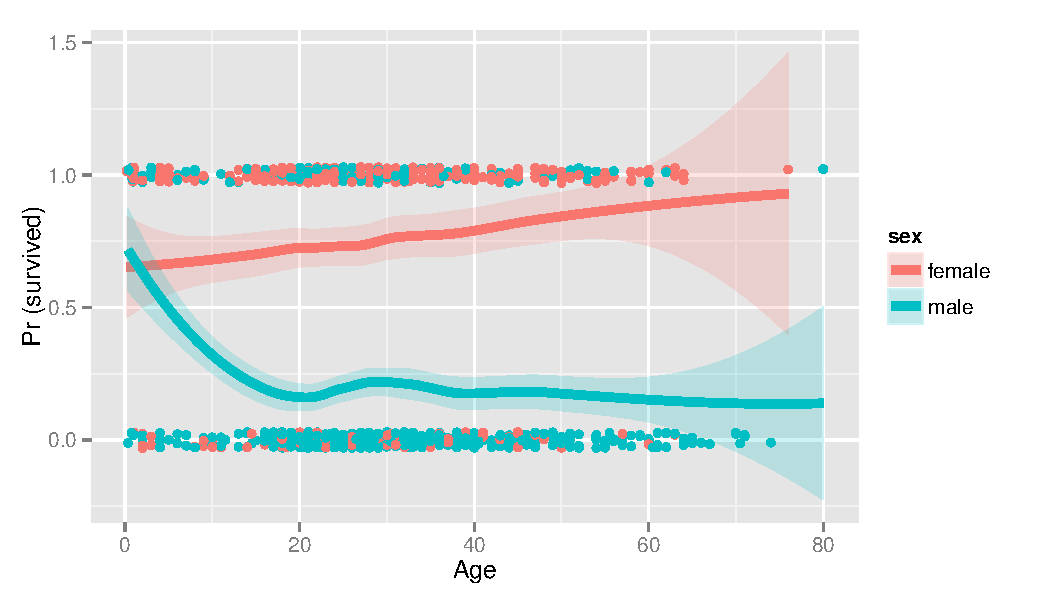
\includegraphics[width=.6\linewidth]{figure/titanic-glm-ggp1} 

}

\caption[Survival on the Titanic, by age and sex, with a \code{loess} smooth and 95\% confidence band]{Survival on the Titanic, by age and sex, with a \code{loess} smooth and 95\% confidence band\label{fig:titanic-glm-ggp1}}
\end{figure}


\end{knitrout}

The points in \figref{fig:titanic-glm-ggp1} show the data; the \code{loess}
curves provide a minimal, but useful summary: among females, survival
rises steadily with \var{age}, while for males, survival appears to
drop precipitously agmong the young and then level off.  The 95\% confidence
bands give a sense of relative precision, and are quite wide for those
over 60 years.

Alternatively, one could use \code{stat\_smooth(method="lm", ...)}
to display the fitted values from a linear probability model,
but here it is of more interest to show the fitted logistic model
(separately for males and females), using
\code{stat\_smooth(method="glm", family=binomial ...)}, as shown in
\figref{fig:titanic-glm-ggp2}.

\begin{knitrout}
\definecolor{shadecolor}{rgb}{0.969, 0.969, 0.969}\color{fgcolor}\begin{kframe}
\begin{alltt}
\hlkwd{ggplot}\hlstd{(Titanicp,} \hlkwd{aes}\hlstd{(age,} \hlkwd{as.numeric}\hlstd{(survived)}\hlopt{-}\hlnum{1}\hlstd{,} \hlkwc{color}\hlstd{=sex))} \hlopt{+}
  \hlkwd{stat_smooth}\hlstd{(}\hlkwc{method}\hlstd{=}\hlstr{"glm"}\hlstd{,} \hlkwc{family}\hlstd{=binomial,} \hlkwc{formula}\hlstd{=y}\hlopt{~}\hlstd{x,}
              \hlkwc{alpha}\hlstd{=}\hlnum{0.2}\hlstd{,} \hlkwc{size}\hlstd{=}\hlnum{2}\hlstd{,} \hlkwd{aes}\hlstd{(}\hlkwc{fill}\hlstd{=sex))} \hlopt{+}
  \hlkwd{geom_point}\hlstd{(}\hlkwc{position}\hlstd{=}\hlkwd{position_jitter}\hlstd{(}\hlkwc{height}\hlstd{=}\hlnum{0.03}\hlstd{,} \hlkwc{width}\hlstd{=}\hlnum{0}\hlstd{))} \hlopt{+}
  \hlkwd{xlab}\hlstd{(}\hlstr{"Age"}\hlstd{)} \hlopt{+} \hlkwd{ylab}\hlstd{(}\hlstr{"Pr (survived)"}\hlstd{)}
\end{alltt}
\end{kframe}\begin{figure}[hb]


{\centering 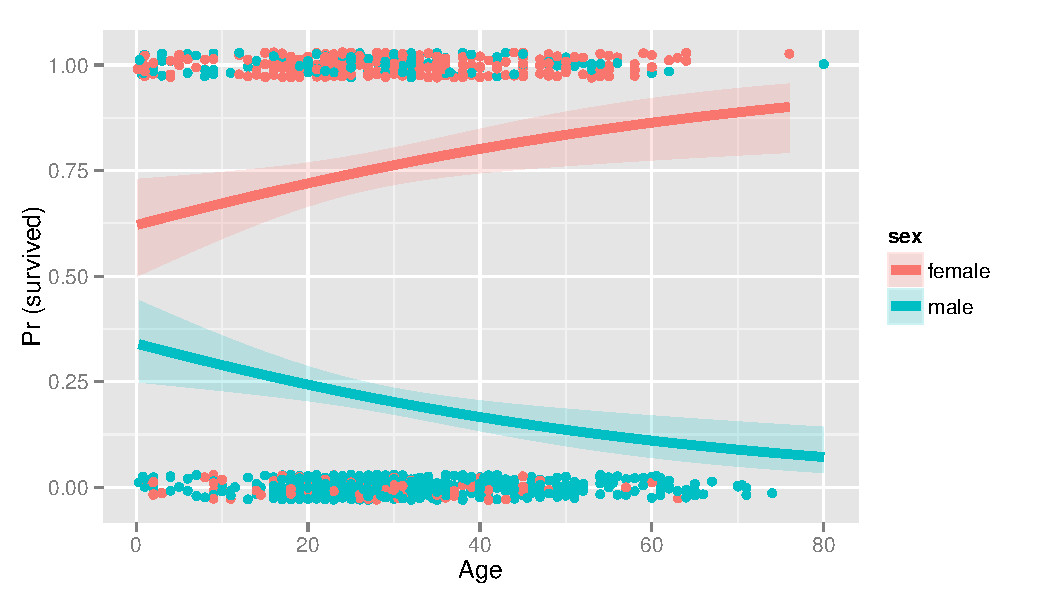
\includegraphics[width=.6\linewidth]{figure/titanic-glm-ggp2} 

}

\caption[Survival on the Titanic, by age and sex, with a \code{glm} smooth and 95\% confidence band]{Survival on the Titanic, by age and sex, with a \code{glm} smooth and 95\% confidence band\label{fig:titanic-glm-ggp2}}
\end{figure}


\end{knitrout}


Showing these results on the scale of probabilities is easier to interpret,
however the relationship between \code{Pr(survived)} and \code{age}
is nonlinear, making it harder to understand interactions in the
more complex models we show below.  One simple way to view the results
on the logit scale is to simply transform the Y axis using
\func{coord\_trans}.  Using this method does not allow the binary observations
to be shown, however, because \code{logit(0)} and \code{logit(1)} are infinite.
\begin{knitrout}
\definecolor{shadecolor}{rgb}{0.969, 0.969, 0.969}\color{fgcolor}\begin{kframe}
\begin{alltt}
\hlstd{logit} \hlkwb{<-} \hlkwa{function}\hlstd{(}\hlkwc{x}\hlstd{)} \hlkwd{log}\hlstd{(x)}\hlopt{/}\hlkwd{log}\hlstd{(}\hlnum{1}\hlopt{-}\hlstd{x)}
\hlkwd{ggplot}\hlstd{(Titanicp,} \hlkwd{aes}\hlstd{(age,} \hlkwd{as.numeric}\hlstd{(survived)}\hlopt{-}\hlnum{1}\hlstd{,} \hlkwc{color}\hlstd{=sex))} \hlopt{+}
  \hlkwd{stat_smooth}\hlstd{(}\hlkwc{method}\hlstd{=}\hlstr{"glm"}\hlstd{,} \hlkwc{family}\hlstd{=binomial,} \hlkwc{formula}\hlstd{=y}\hlopt{~}\hlstd{x,}
              \hlkwc{alpha}\hlstd{=}\hlnum{0.2}\hlstd{,} \hlkwc{size}\hlstd{=}\hlnum{2}\hlstd{,} \hlkwd{aes}\hlstd{(}\hlkwc{fill}\hlstd{=sex))} \hlopt{+}
  \hlkwd{scale_y_continuous}\hlstd{(}\hlkwc{breaks}\hlstd{=}\hlkwd{c}\hlstd{(}\hlnum{.10}\hlstd{,} \hlnum{.25}\hlstd{,} \hlnum{.50}\hlstd{,} \hlnum{.75}\hlstd{,} \hlnum{.90}\hlstd{))} \hlopt{+}
  \hlkwd{coord_trans}\hlstd{(}\hlkwc{y}\hlstd{=}\hlstr{"logit"}\hlstd{)} \hlopt{+} \hlkwd{xlab}\hlstd{(}\hlstr{"Age"}\hlstd{)} \hlopt{+} \hlkwd{ylab}\hlstd{(}\hlstr{"Pr (survived)"}\hlstd{)}
\end{alltt}
\end{kframe}\begin{figure}[hb]


{\centering 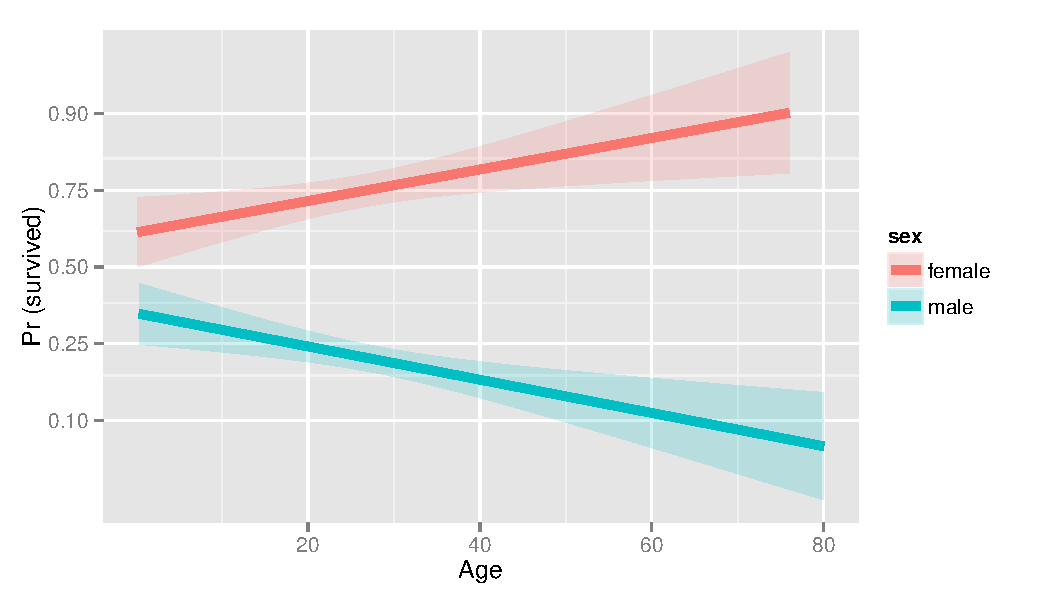
\includegraphics[width=.6\linewidth]{figure/titanic-glm-ggp-logit} 

}

\caption[Survival on the Titanic, by age and sex plotted on the log odds scale where they are linear]{Survival on the Titanic, by age and sex plotted on the log odds scale where they are linear\label{fig:titanic-glm-ggp-logit}}
\end{figure}


\end{knitrout}



These plots don't use passenger class, so this variable is ignored
(or pooled, collapsed over) within each plot and fitted curve.   
Such \glosterm{marginal plots} may be misleading
if there are interactions of \var{pclass} with other variables.
This turns out to be true here, as we will see in Example \texttt{[titanic-eff]}.

One of the strengths
of \pkg{ggplot2} is that it is simple to add faceting by one or two
additional variables to show the same information (points, lines, curves)
in different panels, broken down by those variables for easy comparison.
This is done simply by adding (literally, \code{+} in \R) 
\code{facet\_grid(. \~\ pclass)} to the plot in \figref{fig:titanic-glm-ggp2},
producing \figref{fig:titanic-glm-ggp3}.
\begin{knitrout}
\definecolor{shadecolor}{rgb}{0.969, 0.969, 0.969}\color{fgcolor}\begin{kframe}
\begin{alltt}
\hlstd{p} \hlkwb{<-} \hlkwd{ggplot}\hlstd{(Titanicp,} \hlkwd{aes}\hlstd{(age,} \hlkwd{as.numeric}\hlstd{(survived)}\hlopt{-}\hlnum{1}\hlstd{,} \hlkwc{color}\hlstd{=sex))} \hlopt{+}
  \hlkwd{stat_smooth}\hlstd{(}\hlkwc{method}\hlstd{=}\hlstr{"glm"}\hlstd{,} \hlkwc{family}\hlstd{=binomial,} \hlkwc{formula}\hlstd{=y}\hlopt{~}\hlstd{x,}
              \hlkwc{alpha}\hlstd{=}\hlnum{0.2}\hlstd{,} \hlkwc{size}\hlstd{=}\hlnum{2}\hlstd{,} \hlkwd{aes}\hlstd{(}\hlkwc{fill}\hlstd{=sex))} \hlopt{+}
        \hlkwd{geom_point}\hlstd{(}\hlkwc{position}\hlstd{=}\hlkwd{position_jitter}\hlstd{(}\hlkwc{height}\hlstd{=}\hlnum{0.03}\hlstd{,} \hlkwc{width}\hlstd{=}\hlnum{0}\hlstd{))} \hlopt{+}
        \hlkwd{xlab}\hlstd{(}\hlstr{"Age"}\hlstd{)} \hlopt{+} \hlkwd{ylab}\hlstd{(}\hlstr{"Pr (survived)"}\hlstd{)}
\hlcom{# facet by pclass}
\hlstd{p} \hlopt{+} \hlkwd{facet_grid}\hlstd{(.} \hlopt{~} \hlstd{pclass)}
\end{alltt}
\end{kframe}\begin{figure}[hb]


{\centering 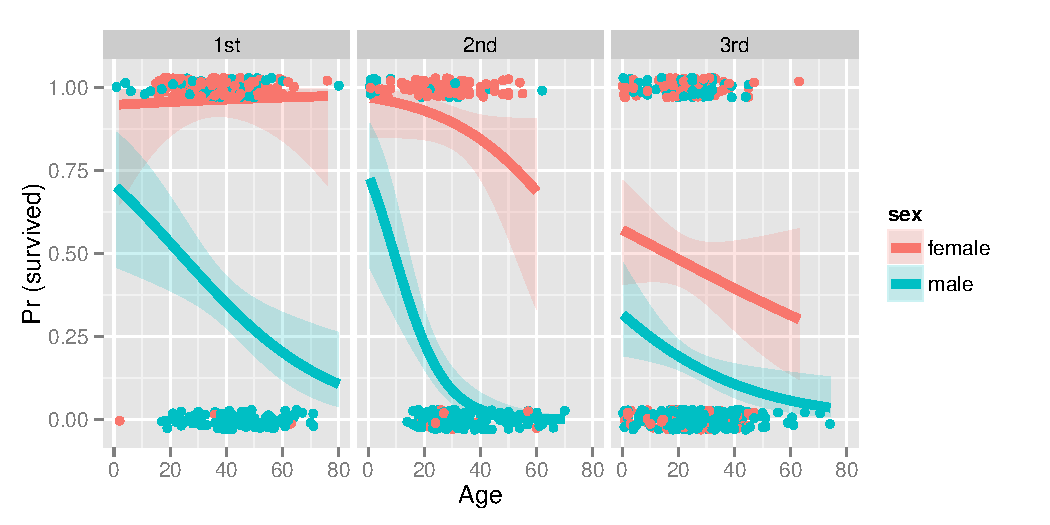
\includegraphics[width=\linewidth]{figure/titanic-glm-ggp3} 

}

\caption[Survival on the Titanic, by age and sex, with panels for passenger class]{Survival on the Titanic, by age and sex, with panels for passenger class\label{fig:titanic-glm-ggp3}}
\end{figure}


\end{knitrout}


For direct comparison with the marginal plot in
\figref{fig:titanic-glm-ggp3}, it is also easy to add the
plot collapsed over \var{pclass} as one more panel in this plot,
by adding the option \code{margins=TRUE}
in the last line in the code above (this plot is not shown).

\begin{knitrout}
\definecolor{shadecolor}{rgb}{0.969, 0.969, 0.969}\color{fgcolor}\begin{kframe}
\begin{alltt}
\hlcom{# add plot collapsed over pclass}
\hlstd{p} \hlopt{+} \hlkwd{facet_grid}\hlstd{(.} \hlopt{~} \hlstd{pclass,} \hlkwc{margins}\hlstd{=}\hlnum{TRUE}\hlstd{)}
\end{alltt}
\end{kframe}
\end{knitrout}


The same type of plot as \figref{fig:titanic-glm-ggp3}
can be produced using facets for \var{sex}, with
separate points and curves within each panel by interchanging
the roles of \var{sex} and \var{pclass} in the code above,
giving \figref{fig:titanic-glm-ggp4}.

\begin{knitrout}
\definecolor{shadecolor}{rgb}{0.969, 0.969, 0.969}\color{fgcolor}\begin{kframe}
\begin{alltt}
\hlcom{# facet by sex, curves by class}
\hlstd{p} \hlkwb{<-} \hlkwd{ggplot}\hlstd{(Titanicp,} \hlkwd{aes}\hlstd{(age,} \hlkwd{as.numeric}\hlstd{(survived)}\hlopt{-}\hlnum{1}\hlstd{,} \hlkwc{color}\hlstd{=pclass))} \hlopt{+}
  \hlkwd{stat_smooth}\hlstd{(}\hlkwc{method}\hlstd{=}\hlstr{"glm"}\hlstd{,} \hlkwc{family}\hlstd{=binomial,} \hlkwc{formula}\hlstd{=y}\hlopt{~}\hlstd{x,}
              \hlkwc{alpha}\hlstd{=}\hlnum{0.2}\hlstd{,} \hlkwc{size}\hlstd{=}\hlnum{2}\hlstd{,} \hlkwd{aes}\hlstd{(}\hlkwc{fill}\hlstd{=pclass))} \hlopt{+}
  \hlkwd{geom_point}\hlstd{(}\hlkwc{position}\hlstd{=}\hlkwd{position_jitter}\hlstd{(}\hlkwc{height}\hlstd{=}\hlnum{0.03}\hlstd{,} \hlkwc{width}\hlstd{=}\hlnum{0}\hlstd{))} \hlopt{+}
        \hlkwd{xlab}\hlstd{(}\hlstr{"Age"}\hlstd{)} \hlopt{+} \hlkwd{ylab}\hlstd{(}\hlstr{"Pr (survived)"}\hlstd{)}
\hlcom{# facet by sex}
\hlstd{p} \hlopt{+} \hlkwd{facet_grid}\hlstd{(.} \hlopt{~} \hlstd{sex)}
\end{alltt}
\end{kframe}\begin{figure}[hbt!]


{\centering 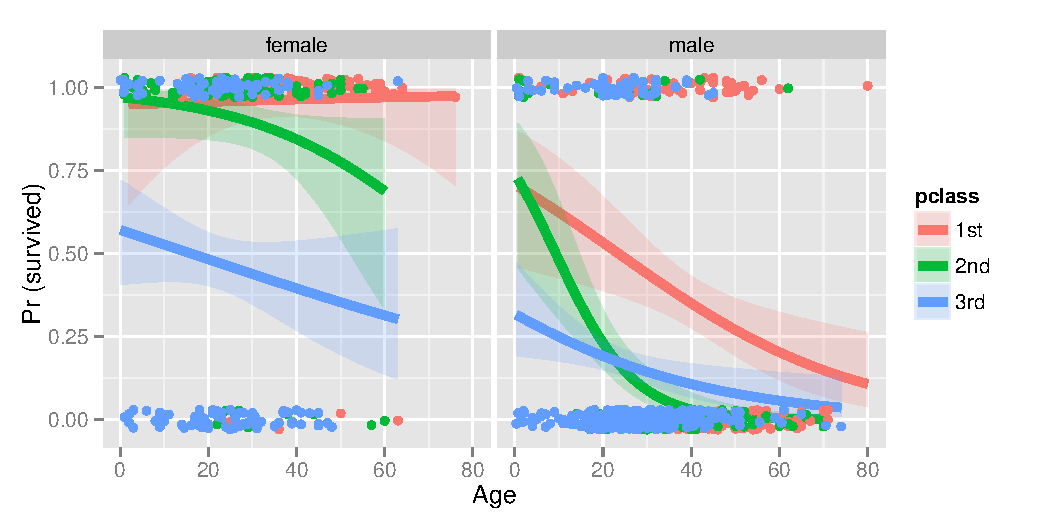
\includegraphics[width=\linewidth]{figure/titanic-glm-ggp4} 

}

\caption[Survival on the Titanic, by age and passenger class, with panels for passenger sex]{Survival on the Titanic, by age and passenger class, with panels for passenger sex\label{fig:titanic-glm-ggp4}}
\end{figure}


\end{knitrout}


The plots above suggest that there are important interactions among the
predictors \var{pclass}, \var{age}, and \var{sex} in their impact on
\var{survival}. In particular, the interaction between 
sex and age appears to differ over passenger class (in \figref{fig:titanic-glm-ggp3}),
and that between passenger class
and age appears to differ between males and females (in \figref{fig:titanic-glm-ggp4})
suggesting a three-way interaction, but this suggestion turns out not to
be supported by the data as we will see below.

One difficulty is that it is hard to determine what constitutes an interaction
 in plots on
the scale of predicted probabilities, where the relations are non-linear. 
As well, such full model plots don't provide any way to tell which apparent
interactions are important.
\end{Example}

\begin{Example}[titanic-eff]{Passengers on the Titanic-- effect plots}

The \Rpackage{effects} provides a simple way to avoid these difficulties,
by calculating and plotting the predicted effects for terms in a given
model, where in any given term (e.g., \code{sex:age}) all low-order relatives
(\code{sex}, \code{age}) are automatically included, and other variables
(e.g., \code{pclass}) are averaged over in a sensible and flexible way.
The function \func{allEffects} in this package identifies all of the
\glossterm{high-order terms} in a given model, and provides plotting methods to visualize
them.  

As well, the plotting functions plot the response variable
(survived) on the logit scale (by default), where relations are assumed to be linear,
but labels the tick marks with their transformed probability values.
Both of these features facilitate interpretation.

But first, we need to determine a reasonable model.

A simple way to proceed is to fit some initial screening models, 
using only main effects, then all two-way terms, \dots, up to the
full model containing all $n$-way effects for $n$ predictors.
The \func{anova} method gives a compact summary of the differences among these.
\begin{knitrout}
\definecolor{shadecolor}{rgb}{0.969, 0.969, 0.969}\color{fgcolor}\begin{kframe}
\begin{alltt}
\hlstd{titanic.glm1} \hlkwb{<-} \hlkwd{glm}\hlstd{(survived} \hlopt{~} \hlstd{pclass} \hlopt{+} \hlstd{sex} \hlopt{+} \hlstd{age,} \hlkwc{data}\hlstd{=Titanicp,} \hlkwc{family}\hlstd{=binomial)}
\hlstd{titanic.glm2} \hlkwb{<-} \hlkwd{glm}\hlstd{(survived} \hlopt{~} \hlstd{(pclass} \hlopt{+} \hlstd{sex} \hlopt{+} \hlstd{age)}\hlopt{^}\hlnum{2}\hlstd{,} \hlkwc{data}\hlstd{=Titanicp,} \hlkwc{family}\hlstd{=binomial)}
\hlstd{titanic.glm3} \hlkwb{<-} \hlkwd{glm}\hlstd{(survived} \hlopt{~} \hlstd{(pclass} \hlopt{+} \hlstd{sex} \hlopt{+} \hlstd{age)}\hlopt{^}\hlnum{3}\hlstd{,} \hlkwc{data}\hlstd{=Titanicp,} \hlkwc{family}\hlstd{=binomial)}
\hlkwd{anova}\hlstd{(titanic.glm1, titanic.glm2, titanic.glm3,} \hlkwc{test}\hlstd{=}\hlstr{"Chisq"}\hlstd{)}
\end{alltt}
\begin{verbatim}
## Analysis of Deviance Table
## 
## Model 1: survived ~ pclass + sex + age
## Model 2: survived ~ (pclass + sex + age)^2
## Model 3: survived ~ (pclass + sex + age)^3
##   Resid. Df Resid. Dev Df Deviance Pr(>Chi)    
## 1      1041        982                         
## 2      1036        918  5     64.6  1.4e-12 ***
## 3      1034        916  2      1.9     0.39    
## ---
## Signif. codes:  0 '***' 0.001 '**' 0.01 '*' 0.05 '.' 0.1 ' ' 1
\end{verbatim}
\end{kframe}
\end{knitrout}

An even more compact summary, including AIC and BIC statistics, may be obtained
using \func{vcdExtra::sumarise} with a \class{glmlist} object:
\begin{knitrout}
\definecolor{shadecolor}{rgb}{0.969, 0.969, 0.969}\color{fgcolor}\begin{kframe}
\begin{alltt}
\hlstd{vcdExtra::}\hlkwd{summarise}\hlstd{(}\hlkwd{glmlist}\hlstd{(titanic.glm1, titanic.glm2, titanic.glm3))}
\end{alltt}
\begin{verbatim}
## Model Summary:
##              LR Chisq   Df Pr(>Chisq)   AIC   BIC
## titanic.glm1      982 1041      0.902 -1100 -5323
## titanic.glm2      918 1036      0.996 -1154 -5357
## titanic.glm3      916 1034      0.996 -1152 -5347
\end{verbatim}
\end{kframe}
\end{knitrout}



From this, we see that the model \code{titanic.glm2} with all two-way terms is
substantially better than the one-way model, and is not improved by adding the
three-way interaction of \code{pclass:sex:age}.  The \func{summary} method for
\class{glm} objects provides details of the goodness of fit of a given model,
and the estimated coefficients, together with signifcance tests.
\begin{knitrout}
\definecolor{shadecolor}{rgb}{0.969, 0.969, 0.969}\color{fgcolor}\begin{kframe}
\begin{alltt}
\hlkwd{summary}\hlstd{(titanic.glm2)}
\end{alltt}
\begin{verbatim}
## 
## Call:
## glm(formula = survived ~ (pclass + sex + age)^2, family = binomial, 
##     data = Titanicp)
## 
## Deviance Residuals: 
##    Min      1Q  Median      3Q     Max  
## -2.614  -0.675  -0.443   0.377   3.245  
## 
## Coefficients:
##                   Estimate Std. Error z value Pr(>|z|)    
## (Intercept)        3.39036    0.80528    4.21  2.6e-05 ***
## pclass2nd          0.76467    0.95984    0.80  0.42565    
## pclass3rd         -3.27000    0.76482   -4.28  1.9e-05 ***
## sexmale           -2.59223    0.75357   -3.44  0.00058 ***
## age               -0.00395    0.01757   -0.22  0.82216    
## pclass2nd:sexmale -0.87884    0.68994   -1.27  0.20274    
## pclass3rd:sexmale  1.88570    0.58463    3.23  0.00126 ** 
## pclass2nd:age     -0.06053    0.02142   -2.83  0.00471 ** 
## pclass3rd:age     -0.00624    0.01619   -0.39  0.69971    
## sexmale:age       -0.03138    0.01512   -2.08  0.03793 *  
## ---
## Signif. codes:  0 '***' 0.001 '**' 0.01 '*' 0.05 '.' 0.1 ' ' 1
## 
## (Dispersion parameter for binomial family taken to be 1)
## 
##     Null deviance: 1414.62  on 1045  degrees of freedom
## Residual deviance:  917.84  on 1036  degrees of freedom
## AIC: 937.8
## 
## Number of Fisher Scoring iterations: 5
\end{verbatim}
\end{kframe}
\end{knitrout}

In general, I don't find these numerical results particularly useful for interpretation.
\var{pclass} and \var{age} are factors, and so the coefficients of
terms involving them relate to the parameterization used by \func{glm}, 
which here is the (default) \func{contr.treatment}, where the first level of a factor
is the baseline, against which the others are compared.%
\footnote{
In this example, \var{pclass} should arguably be treated as an \emph{ordered} factor,
so that differences among the passenger classes are resolved into linear trends
(slopes) and quadratic trends (curvature) on the logit scale. This can be done by
re-assigning \var{pclass} globally as an ordered factor,
\code{Titanicp\$pclass <- ordered(Titanicp\$pclass)}, or better yet, by using
the option \code{contrasts=list(pclass=contr.poly)}  in the call to \func{glm}
to use \func{contr.poly} locally within this call.  
The parameterization used makes no difference in overall tests of model effects or
in model-based plots, but does make a difference for interpretation of parameter values.
}
\begin{knitrout}
\definecolor{shadecolor}{rgb}{0.969, 0.969, 0.969}\color{fgcolor}\begin{kframe}
\begin{alltt}
\hlkwd{contrasts}\hlstd{(Titanicp}\hlopt{$}\hlstd{pclass)}
\end{alltt}
\begin{verbatim}
##     2nd 3rd
## 1st   0   0
## 2nd   1   0
## 3rd   0   1
\end{verbatim}
\end{kframe}
\end{knitrout}


The \func{Anova} function in the \Rpackage{car} gives a more useful and compact summary
here, 
\begin{knitrout}
\definecolor{shadecolor}{rgb}{0.969, 0.969, 0.969}\color{fgcolor}\begin{kframe}
\begin{alltt}
\hlkwd{Anova}\hlstd{(titanic.glm2)}
\end{alltt}
\begin{verbatim}
## Analysis of Deviance Table (Type II tests)
## 
## Response: survived
##            LR Chisq Df Pr(>Chisq)    
## pclass        121.5  2    < 2e-16 ***
## sex           275.8  1    < 2e-16 ***
## age            34.9  1    3.4e-09 ***
## pclass:sex     38.2  2    5.2e-09 ***
## pclass:age     10.1  2     0.0065 ** 
## sex:age         4.3  1     0.0374 *  
## ---
## Signif. codes:  0 '***' 0.001 '**' 0.01 '*' 0.05 '.' 0.1 ' ' 1
\end{verbatim}
\end{kframe}
\end{knitrout}


From this, we can proceed to visualize the predicted effects for the three two-way interactions 
in the \code{titanic.glm2} model.  \func{allEffects} calculates the fitted values for each
term and returns a \class{efflist} object, a list of \class{eff} objects for the terms.
\begin{knitrout}
\definecolor{shadecolor}{rgb}{0.969, 0.969, 0.969}\color{fgcolor}\begin{kframe}
\begin{alltt}
\hlkwd{library}\hlstd{(effects)}
\hlstd{titanic.eff2} \hlkwb{<-} \hlkwd{allEffects}\hlstd{(titanic.glm2)}
\hlkwd{names}\hlstd{(titanic.eff2)}
\end{alltt}
\begin{verbatim}
## [1] "pclass:sex" "pclass:age" "sex:age"
\end{verbatim}
\end{kframe}
\end{knitrout}

\func{allEffects} is very general in how variables not included in a given term
are represented.  By default, these other columns of the model matrix
are averaged over (\code{typical=mean}) and factors such as \var{pclass} and
\var{sex} are represented by their proportions in the data.  These options
can be changed as shown below, to use the median value, and to calculate predicted
effects for equal proportions of class and sex.

\begin{knitrout}
\definecolor{shadecolor}{rgb}{0.969, 0.969, 0.969}\color{fgcolor}\begin{kframe}
\begin{alltt}
\hlstd{titanic.eff2a} \hlkwb{<-} \hlkwd{allEffects}\hlstd{(titanic.glm2,}
  \hlkwc{typical}\hlstd{=median,}
  \hlkwc{given.values}\hlstd{=}\hlkwd{c}\hlstd{(}\hlkwc{pclass2nd}\hlstd{=}\hlnum{1}\hlopt{/}\hlnum{3}\hlstd{,} \hlkwc{pclass3rd}\hlstd{=}\hlnum{1}\hlopt{/}\hlnum{3}\hlstd{,} \hlkwc{sexmale}\hlstd{=}\hlnum{0.5}\hlstd{)}
        \hlstd{)}
\end{alltt}
\end{kframe}
\end{knitrout}


For interactive use, it is easy to plot various terms using a menu to select
the high-order terms to be plotted; \code{...} stands for other arguments
to control these plots.
\begin{knitrout}
\definecolor{shadecolor}{rgb}{0.969, 0.969, 0.969}\color{fgcolor}\begin{kframe}
\begin{alltt}
\hlkwd{plot}\hlstd{(titanic.eff2,} \hlkwc{ask}\hlstd{=}\hlnum{TRUE}\hlstd{, ...)}
\end{alltt}
\end{kframe}
\end{knitrout}

Below we plot these terms separately, using some options to control the plots.
In particular, \code{multiline=TRUE} plots the levels of a factor within a
single plot to make visual comparison easier, rather than using a multi-panel display.
By default, this suppresses confidence intervals, so we turn that back on
using \code{ci.style="bars"}.

The first term, showing the \code{pclass*sex} effect can be plotted as follows:
\begin{knitrout}
\definecolor{shadecolor}{rgb}{0.969, 0.969, 0.969}\color{fgcolor}\begin{kframe}
\begin{alltt}
\hlstd{ticks} \hlkwb{<-} \hlkwd{list}\hlstd{(}\hlkwc{at}\hlstd{=}\hlkwd{c}\hlstd{(}\hlnum{.01}\hlstd{,} \hlnum{.05}\hlstd{,} \hlkwd{seq}\hlstd{(}\hlnum{.1}\hlstd{,} \hlnum{.9}\hlstd{,} \hlkwc{by}\hlstd{=}\hlnum{.2}\hlstd{),} \hlnum{.95}\hlstd{,} \hlnum{.99}\hlstd{))}
\hlkwd{plot}\hlstd{(titanic.eff2[}\hlnum{1}\hlstd{],} \hlkwc{ticks}\hlstd{=ticks,} \hlkwc{multiline}\hlstd{=}\hlnum{TRUE}\hlstd{,} \hlkwc{ci.style}\hlstd{=}\hlstr{"bars"}\hlstd{,} \hlkwc{key}\hlstd{=}\hlkwd{list}\hlstd{(}\hlkwc{x}\hlstd{=}\hlnum{.7}\hlstd{,} \hlkwc{y}\hlstd{=}\hlnum{.95}\hlstd{))}
\end{alltt}
\end{kframe}

{\centering 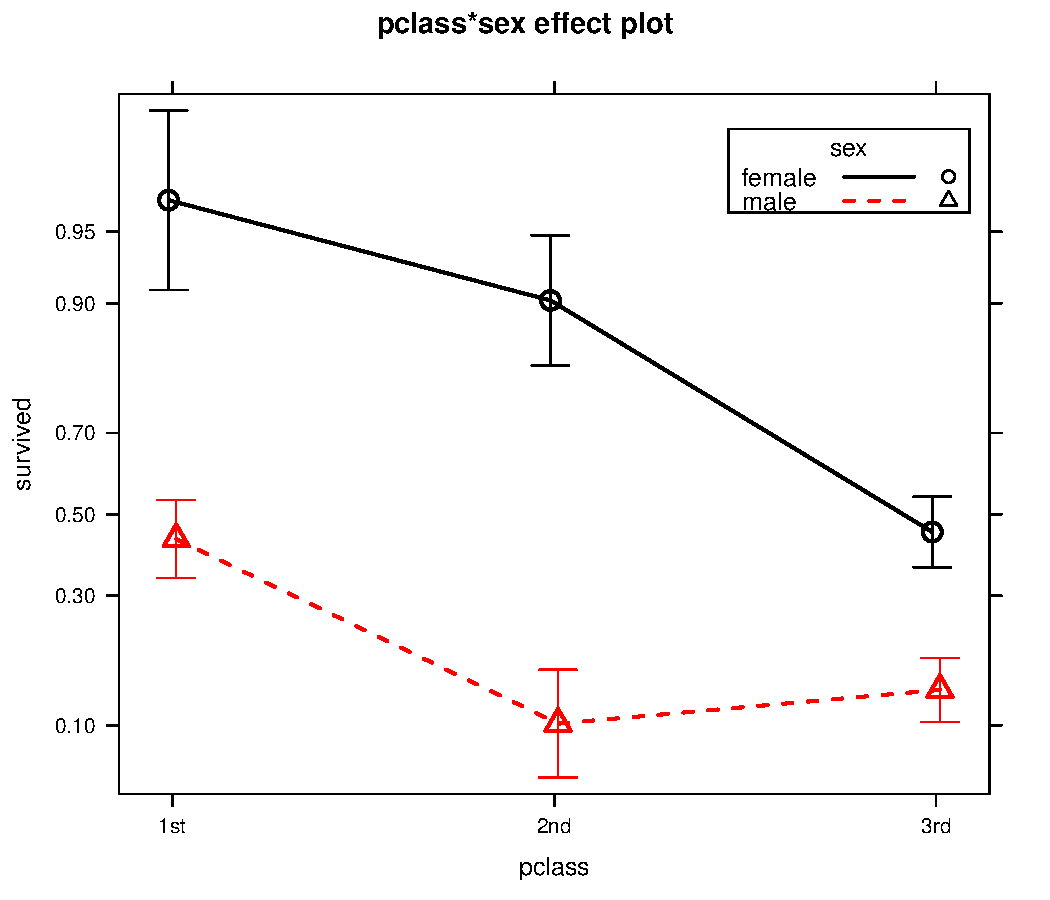
\includegraphics[width=.5\linewidth]{figure/titanic-eff2-1} 

}



\end{knitrout}

It can be seen directly that although women were, overall, more likely to survive than
men, the difference in survival between the sexes in 3$^{rd}$ class were much smaller
than in 1$^{st}$ or 2$^{nd}$ class, which explains the \code{pclass:sex} interaction.

The other two terms plotted in the same way:
\begin{knitrout}
\definecolor{shadecolor}{rgb}{0.969, 0.969, 0.969}\color{fgcolor}\begin{kframe}
\begin{alltt}
\hlkwd{plot}\hlstd{(titanic.eff2[}\hlnum{2}\hlstd{],} \hlkwc{ticks}\hlstd{=ticks,} \hlkwc{multiline}\hlstd{=}\hlnum{TRUE}\hlstd{,} \hlkwc{ci.style}\hlstd{=}\hlstr{"bars"}\hlstd{,} \hlkwc{key}\hlstd{=}\hlkwd{list}\hlstd{(}\hlkwc{x}\hlstd{=}\hlnum{.7}\hlstd{,} \hlkwc{y}\hlstd{=}\hlnum{.95}\hlstd{))}
\end{alltt}
\end{kframe}
\end{knitrout}

\begin{knitrout}
\definecolor{shadecolor}{rgb}{0.969, 0.969, 0.969}\color{fgcolor}\begin{kframe}
\begin{alltt}
\hlkwd{plot}\hlstd{(titanic.eff2[}\hlnum{3}\hlstd{],} \hlkwc{ticks}\hlstd{=ticks,} \hlkwc{multiline}\hlstd{=}\hlnum{TRUE}\hlstd{,} \hlkwc{ci.style}\hlstd{=}\hlstr{"bars"}\hlstd{,} \hlkwc{key}\hlstd{=}\hlkwd{list}\hlstd{(}\hlkwc{x}\hlstd{=}\hlnum{.7}\hlstd{,} \hlkwc{y}\hlstd{=}\hlnum{.95}\hlstd{))}
\end{alltt}
\end{kframe}
\end{knitrout}


%% two figs side by side
\begin{figure}[htb!]
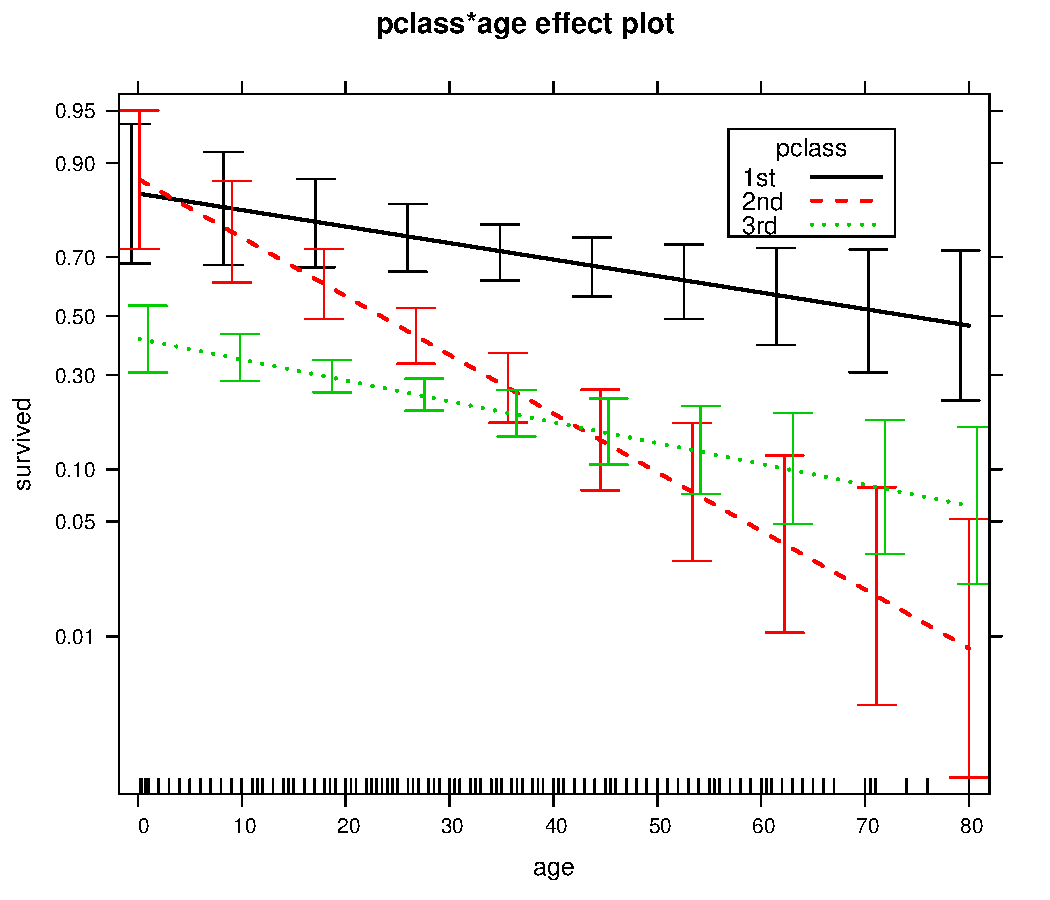
\includegraphics[width = .49\linewidth]{figure/titanic-eff2-2}
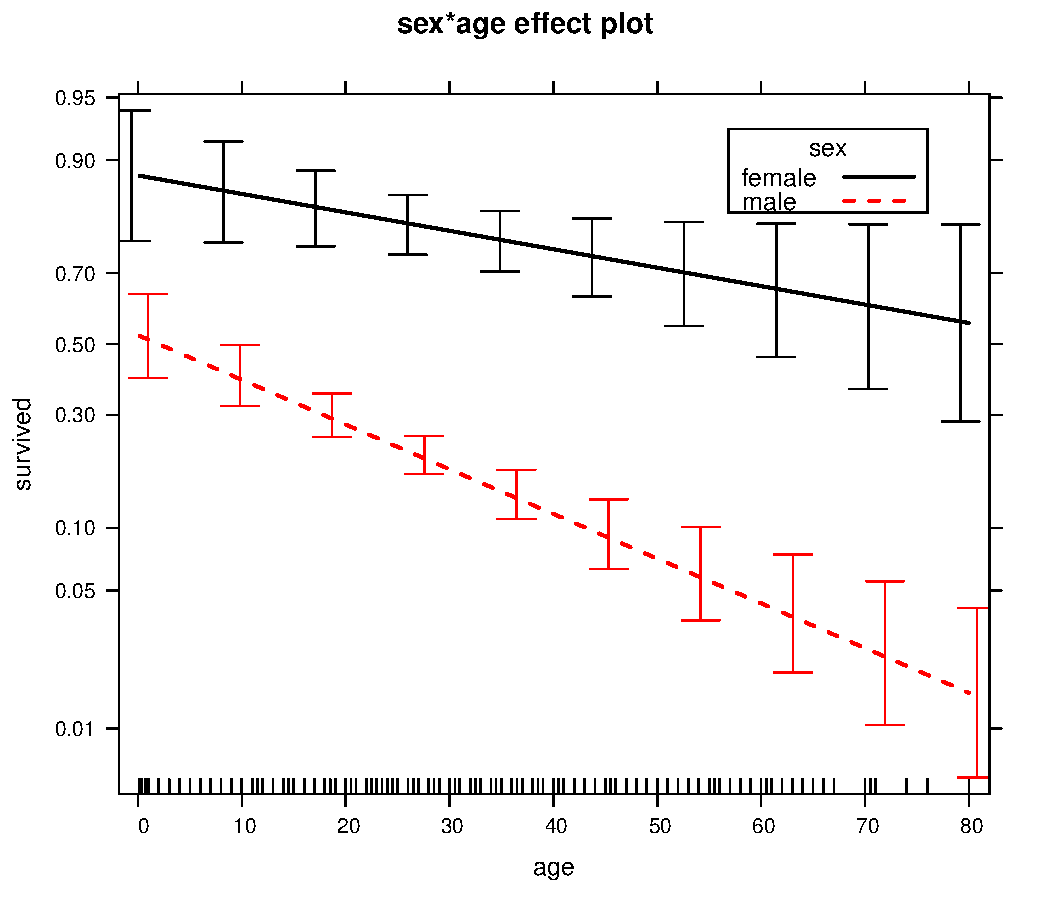
\includegraphics[width = .49\linewidth]{figure/titanic-eff2-3}
\caption{Effect plots for two-way interactions in the model \texttt{titanic.glm2}.
These plots show the predicted value of the log odds of survival for the two
variables shown in each plot, averaged over the remaining variable.}
\label{fig:titanic-eff2-23}
\end{figure}

The interpretation of the results from these plots is much simpler than from 
a table of coefficients or even than from the full model plots shown earlier.
In \figref{fig:titanic-eff2-23} (left) it can be seen that while survival
in all classes decreased with age, and survival decreased overall with lower
class, the effect of age on survival was much greater in 2$^{nd}$ class-- a steeper
negative slope.

% here, we need \dorefs from command.sty, allowing Figure 1,2 and 4.

The right panel of \figref{fig:titanic-eff2-23}
shows the \code{sex*age} effect that we have seen in earlier
figures (\figref{fig:titanic-glm-ggp2} and \figref{fig:titanic-glm-ggp-logit}),
but with one crucial difference (that argues strongly for effect plots):
In the earlier full model
plots, passenger class was not controlled (or adjusted for),
so the apparent tendency of older female passengers to be more likely
to survive than younger ones is due in part to the different distributions
of passenger class across sex and age.
A correct interpretation of the \code{sex*age} effect is that
controlling for passenger class,
for both genders, survival decreased with age, but not as
much for women as for men.


\end{Example}
\end{document}
